% =====================================================================
% FaithfulProse --- arXiv preprint
% Faithful on Prose, Unanchored on Reasoning:
%   A Position-Domain Calibration of the Jacobian Lens
%
% Canonical index : FaithfulProse/LINKS.md
% Frozen sources  : DESIGN_c_lens_pos_v2 / PREREG_r2 / PREREG_r3
% All numbers come from the released JSON artifacts; see Sec. Data.
% =====================================================================
\documentclass[11pt]{article}

\usepackage[T1]{fontenc}
\usepackage[utf8]{inputenc}
\usepackage[margin=1in]{geometry}
\usepackage{amsmath,amssymb}
\usepackage{graphicx}
\usepackage{booktabs}
\usepackage{caption}
\usepackage{microtype}
\usepackage[hidelinks]{hyperref}
\usepackage{url}

\graphicspath{{figs/}}

% Public repository. Must be public at submission time (the Data availability
% URL would otherwise 404).
\newcommand{\REPOURL}{\url{https://github.com/moyhig-ecs/FaithfulProse}}
% Archive DOI. Until it is minted, leave the macro at its placeholder AND keep
% \DOICLAUSE empty: `make check` then refuses to pass, while the placeholder is
% never rendered into the PDF. (An earlier build published the placeholder.)
% v1.0.0: 10.5281/zenodo.21768365 (filled 2026-08-03). v2: the VERSION DOI of the
% v2.0.0: 10.5281/zenodo.22041132 (filled 2026-08-21). VERSION DOI, pins the bytes of v2.0.0.
% The concept DOI --- all versions, always resolving to the latest --- is
% 10.5281/zenodo.21768364 and is deliberately not the one cited here.
% v3.0.0: 10.5281/zenodo.22219123 (filled 2026-09-01). VERSION DOI, pins the bytes of v3.0.0
% v3.1.0: 10.5281/zenodo.22928427 (filled 2026-09-24). VERSION DOI, pins the bytes of v3.1.0 (refitted-lens re-reads)
% (the TSD-20260826 re-acquisition). Concept DOI 21768364 is deliberately not the one cited here.
\newcommand{\REPODOI}{10.5281/zenodo.22928427}
\newcommand{\DOICLAUSE}{, archived at \href{https://doi.org/\REPODOI}{\texttt{\REPODOI}}}
\captionsetup{font=small,labelfont=bf}

\title{\bfseries Faithful on Prose, Unanchored on Reasoning:\\
A Position-Domain Calibration of the Jacobian Lens}

\author{Manabu Higashida\\
\small D3 Center, The University of Osaka, Osaka, Japan\\
\small \texttt{manabu.higashida.cmc@osaka-u.ac.jp} \quad ORCID: 0009-0004-7393-2957}

\date{\small Version 3.2 (REVISION-ID: TSD-20260826), 2026-09-23}

\begin{document}
\maketitle

\begin{abstract}
\noindent
The Jacobian lens (J-lens) reads which tokens a language model is
positioned to verbalize, and its released artifacts are being inherited
as defaults. Those artifacts are fitted with a maximum sequence length of
128 tokens, a setting that appears in the distributed configuration files
and not in the main text of the canonical write-up --- and 128 is also the
default of the published fitting script, so it propagates to independently
fitted lenses as well; readers are applying the lens
thousands of tokens deep. We calibrate fidelity against position on
OLMo-3-32B, with the decision table, the thresholds, and the axes of both
figures committed before any measurement existed. On prose --- the lens's
home domain --- fidelity does not decay with depth. On reasoning traces
it does, but the finding does not survive contact with its own
coordinate system: the same measurements read as a degradation of
$+0.82$ dex against one baseline cell and an improvement of $-0.14$ dex
against another. We report both coordinates and treat that dependence as
a primary result rather than a nuisance. Extending the prompt axis from
one prompt to three, we find the deep-prompt degradation reproduces in
all three, and that in two of them the decision is carried by a
deep-rank measure alone while head-of-distribution rank correlation
stays flat --- the failure mode we had named at design time in order to
guard against it. A second campaign holds a short two-hop prompt fixed and translates it in depth behind a content-free corridor of filler, so that one read-out can be followed across the fit boundary without changing what is read. Across corridor lengths from 88 to 484 tokens, the landmark-relative onset of the read-out is unchanged in every cell that passes a frozen behavioral-invariance gate. We state this as a scope-qualified absence, not a calibration: an instrument that did not break out of its domain has not thereby been calibrated there. We give the resulting problem a name: \emph{the
calibration was anchored neither outside nor inside the instrument} ---
no external oracle to check it against, and no internal origin to
measure from. The two halves differ in kind. The missing external oracle
is structural: an instrument that reads disposition can only be checked
against next-token logits, which differ by construction from what it
reads, and that carries to any disposition-reading instrument checked the
same way. The
missing internal origin is a single measured instance, on this lens and
this axis, and we do not claim it generalizes. We also do not claim the
lens is unusable: on prose it is faithful. The claim is narrower and, we
think, more useful: readings taken deep inside a reasoning trace have no
verifiable anchor. That absence of an anchor is not specific to this
lens --- anyone
who inherits a disposition-reading instrument together with its default
settings inherits the same problem. Give us a ruler for the order of
reasoning.
\end{abstract}

\vspace{0.4em}
\noindent\textbf{Keywords:} interpretability; Jacobian lens; calibration;
position domain; pre-registration; language models

% =====================================================================
\section{Introduction}
\label{sec:intro}

The Jacobian lens (J-lens) was introduced by Gurnee et al.\ as an
instrument for identifying internal representations that are readily
available for verbal report~\cite{gurnee2026workspace}. For each token in
the vocabulary, ``the Jacobian lens identifies a vector representation
that encodes the potential for the model to verbalize that token in the
future''~\cite{gurnee2026workspace}. Collectively these vectors are
termed the \emph{J-space}. Fitted lenses have been released publicly for
several models, and downstream work --- ours included --- has begun to
use them.

An instrument that ships with defaults will be used with those defaults.
This paper asks a question that the instrument's own documentation does
not answer: \emph{over what range of token positions is the lens
calibrated?}

The canonical write-up describes the fit as an expectation ``over the
source position $t$, all subsequent positions $t'$ within the context,
and a corpus of one thousand prompts sampled from a pretraining-like
distribution''~\cite{gurnee2026workspace}. Its main text states neither the
sequence length used in fitting nor any dependence of fidelity on token
position within the context.\footnote{The write-up does note that readouts
are noisy in early \emph{layers}; that concerns depth in the network, not
position within the sequence.}\footnote{We searched the published page on
2026-08-03 for \texttt{max\_seq}, \texttt{max\_seq\_len}, ``sequence
length'', ``context length'', ``context window'', ``token limit'', ``prompt
length'', ``truncat'' and ``window size''; none occurs. We were not able to
retrieve the appendices, so this is a statement about the main text only. The
search predicates, the date and this limitation are recorded with the release.} The actual setting ---
\texttt{max\_seq\_len} $=128$ --- appears only in the configuration files
distributed alongside the fitted lenses, and it is the same across all
six released lenses. A user therefore cannot learn the position domain
from the paper; they learn it by opening a config file.

We do not present this as a defect of the original work: a research note
may reasonably omit such a parameter. We present it as a fact with a
consequence. The position domain is inherited undocumented, and the
distance between where the lens was fitted (128 tokens) and where it is
applied (we ourselves had been reading at 8192) is a factor of 64; this
study measures out to 16384, a factor of 128.

This paper calibrates that gap and reports what calibration could and
could not establish. Section~\ref{sec:method} describes a procedure whose
central feature is that the decision table and both figure frames were
frozen and committed before any measurement existed.
Section~\ref{sec:results} reports the measurements.
Section~\ref{sec:contribution} states what we take to be the main
contribution, which is not a number.

Our position is a calibration, not a rejection. The original authors are
explicit that ``the Jacobian lens is an imperfect tool, which we believe
only approximately and incompletely captures the model's underlying
workspace structure''~\cite{gurnee2026workspace}. This work is in the
same direction as that sentence.

This version adds a second campaign (Sections~\ref{sec:campaign2}, \ref{sec:arms} and \ref{sec:results2}) and records a second edge of the fit domain (Section~\ref{sec:method}). Nothing from version 1.1 is withdrawn; the new material is additive, and the version history is kept with the archive. Version 3.0 (REVISION-ID: TSD-20260826) re-acquires every reading-set measurement of the second campaign under a repaired token-set acceptance; what changed, what was re-measured and what is newly registered are listed in the Revision History section, and the superseded readings are marked inline. Version 3.1 changes no value: it declares, in the Revision History, the instrument state under which the re-acquisition actually ran. Version 3.2 withdraws no value either: it adds an instrument-provenance note (Section~\ref{sec:provenance-note}) and places the readings of the refitted lens beside the June readings.

% =====================================================================
\section{Method}
\label{sec:method}

\subsection{Calibration target}

\begin{center}
\small
\begin{tabular}{@{}lp{12.6cm}@{}}
\toprule
Lens & J-lens, public artifact, 2026-06-16 fit (md5 \texttt{c73a32d1\ldots}); fitted under transformers 5.11.0 --- see \S\ref{sec:provenance-note} \\
Read-out forward & transformers 5.14.1 (post huggingface/transformers\#46911) \\
Model & OLMo-3-1125-32B, bfloat16, no chat template \\
Read-out band & layers 26--56 (31 layers: 8 full-attention, 23 sliding) \\
Fit setting & \texttt{max\_seq\_len} $=128$; \texttt{wikitext-103-raw-v1} \\
Fit positions & $[16, 128)$: the fitting script skips the first 16 positions (\texttt{SKIP\_FIRST\_N\_POSITIONS} $=16$) \\
Prior use & our earlier runs applied it at \texttt{max\_seq\_len} $=8192$ \\
\bottomrule
\end{tabular}
\end{center}

The fit domain has two edges, and both live in the same file. The fitting script skips the first sixteen positions of every sequence --- its comment reads ``early positions act as attention sinks and have atypical residual statistics'' --- and caps the sequence at 128; neither number is in the main text of the canonical write-up. Version 1.1 treated only the upper edge. The lower edge matters for two of the checks below, and we mark where it does. A companion note under the same frozen protocol (FidelityEight~\cite{fidelityeight2026}) measures the distributed 32B lens against its model on a fixed 266-item prose set: a median word-group rank deviation of 1.57 dex, against a chance floor of 4.47 dex and a vanilla-logit-lens baseline of 1.84 dex on the 7B ground; binding the read-out to the lens's own fit positions ($\geq 16$) moves these by at most 0.10 dex. Those are absolute readings of the instrument. This paper remains about their dependence on position.

\subsection{Quantities: calibrate on what the instrument consumes}

A calibration is only as good as its choice of measured quantity. We
report five.

\begin{center}
\small
\begin{tabular}{@{}ll@{}}
\toprule
$\mathrm{KL}$ & $\mathrm{KL}(\mathrm{softmax}(\text{model})\,\|\,\mathrm{softmax}(\text{lens}))$, band median \\
top-1 & argmax agreement, band mean \\
Rank correlation & Spearman on the model's top-$K$ ($K=1000$), band median \\
\textbf{Word-group rank deviation} & $|\log_{10}\text{rank}_{\text{lens}} - \log_{10}\text{rank}_{\text{model}}|$, band median \\
Baseline contrast & the same, against a vanilla logit lens~\cite{nostalgebraist2020logitlens} \\
\bottomrule
\end{tabular}
\end{center}

The fourth quantity requires comment, because it is the one that
ultimately decided this paper. Rank correlation over the model's top-1000
measures fidelity at the \emph{head} of the distribution. The downstream
use we care about --- reading which of two word groups is ranked higher
--- consumes ranks that lie two to five orders of magnitude deep. Head
fidelity does not guarantee depth fidelity: a lens whose head is faithful
and whose flank is distorted could pass a decision table built on rank
correlation alone. We therefore added \emph{word-group rank deviation} as
a fifth quantity at design time, and made the decision the worst of
$\{$rank correlation, word-group rank deviation$\}$, specifically to
guard against that failure mode. Section~\ref{sec:pdepth} reports what
happened.

\subsection{The freezing procedure}
\label{sec:freeze}

The methodological commitment of this paper is procedural:

\begin{enumerate}\itemsep2pt
\item The decision table --- thresholds, decision group, baseline,
  minimum cell sizes --- was frozen and committed \emph{before}
  measurement.
\item The figures' axes, bucket boundaries and decision lines were
  frozen and committed while no data point existed: the plotting scripts
  draw an empty frame if the results file is absent.
\item When results arrived, the table was applied mechanically. The
  operator moved neither a threshold nor a verdict.
\item Where data did not fit the frozen frame, the frame was not widened.
  Out-of-range points are marked with triangles and their values printed.
\end{enumerate}

Each commit timestamp is verifiable evidence that the freeze preceded the
measurement. The procedure fired twice during this study. Once, the
frozen figure axis (an absolute $\Delta$ in dex) caught a unit mismatch
in the prose of the decision table (a ratio with a floor); the frame was
right and the text was corrected to match it. Once, data exceeded the
frozen limits in both directions and was received with triangles rather
than a wider axis --- so that ``it did not fit'' survived as information.

\subsection{Sample}
\label{sec:sample}

\begin{center}
\small
\begin{tabular}{@{}ll@{}}
\toprule
Prose corpus (W) & 4 concatenated \texttt{wikitext-103}~\cite{merity2017wikitext} texts, $\geq$16{,}400 tokens each \\
 & (the lens's fit dataset; article boundaries recorded in provenance) \\
Reasoning traces (G) & 8 generation traces over 3 prompts: \\
 & \quad prompt 1 (458 tokens) --- 2 traces \\
 & \quad prompt 2 (470 tokens) --- 2 traces \\
 & \quad prompt 3 (501 tokens) --- 4 traces \\
Positions & 8 evenly spaced per frozen bucket; one forward pass reads all \\
Total & 924 measurements (700 initial $+$ 224 in the multi-prompt extension) \\
\bottomrule
\end{tabular}
\end{center}

The three prompts are edit variants of one base task and therefore share
prefixes: prompt 3 diverges from prompts 1 and 2 at token 86, and prompts
1 and 2 diverge from each other at token 354. Limitation~3
(\S\ref{sec:limits}) treats the consequences, which are substantial.

The sampling rule for the extension was itself frozen before the run:
scanning seeds in ascending order, take the first two traces with more
than 512 tokens. The length cutoff is not arbitrary but a requirement of
the position grid --- a shorter trace has its bucket ceilings truncated,
so the same absolute positions can no longer be compared across prompts.
One candidate trace was disqualified by this rule.

\subsection{Reproducibility and positive controls}

\begin{center}
\small
\begin{tabular}{@{}ll@{}}
\toprule
Two applications, identical settings & all values $\Delta = 0$; ranks 48/48 identical \\
Same, with truncation active & all values $\Delta = 0$; ranks 47/47 identical \\
Implementation difference at equal length & word-group rank deviation, median 0.0109 dex \\
\textbf{Control A} (aggregator) & reproduces the published re-aggregation: 170 values, 0 differing \\
\textbf{Control B} (measurement) & reproduces a certified trace: 520 values, 0 differing \\
\bottomrule
\end{tabular}
\end{center}

Read-out is deterministic, and the implementation difference is below
half the decision threshold. For the multi-prompt extension we did not
assume that the extension's instrument was a faithful copy of the frozen
one; we measured it, with Controls A and B, before taking any new
measurement. A mismatch in either was a pre-registered stopping condition
that would have halted the run before it began.

One caveat belongs here. Prompt-side read-outs agree \emph{exactly} only
when the run configuration --- the set of positions read together, and
the sequence length --- also agrees. Across pairs differing only in run
configuration, with prompt and prefix identical, we observed a median of
0.009 dex and a maximum of 0.031 dex, one tenth of the decision threshold
($n = 15$ positions, single prompt pair). We do not identify a mechanism.

\subsection{Second campaign: instrument checks and a depth translation}

\label{sec:campaign2}

Version 1.1 measured fidelity against the model's logits along the position axis, and that comparison has no external anchor (Section~\ref{sec:contribution}). The second campaign asks a different question, one that needs no ground truth: if the content of a prompt is held fixed and only its depth in the sequence is changed, does a read-out taken from it move? We call the resulting series MapFirst (the map of the instrument comes first; any claim about the model is made on top of it). The prompts come from a companion program, SilentHop (the silent hop: the unverbalized intermediate of a multi-hop query, read at prompt positions with a calibrated lens --- that is, inside the domain this paper measures), whose substantive findings are not reported here; we use its first three arms --- Arm A (a positive control read at the head of the sequence, below position 16), Arm B and Arm C --- only as instrument checks, and MapFirst as their extension across the fit boundary, where everything is descriptive (Section~\ref{sec:results2}). Every arm was pre-registered with its predicates, thresholds and stopping rules frozen and committed before it ran, as in Section~\ref{sec:freeze}; all runs are single forward passes on the same lens (md5 \texttt{c73a32d1\ldots}), the same read-out band and the same model as version 1.1.

\paragraph{Read-out.} Each prompt is a two-hop question whose intermediate entity is never verbalized; there are five prompts of 10--14 tokens, each with two distractor entities (for the row whose intermediate is Canada, the answer is Ottawa and the distractors are Toronto and Washington). The read-out is the band-median rank (layers 26--56) of the intermediate's token at each position. A row \emph{rises} when the intermediate ranks above both distractors for three consecutive positions ($k = 3$); its \emph{onset} is the first position of that window, reported relative to a landmark --- the first token of the question proper --- so that prompts at different depths can be compared. The onset is the position at which the intermediate becomes readable by this lens; we do not read it as the time at which anything is computed.

\paragraph{Gate and controls.} Three frozen devices carry the campaign. (i) A \emph{behavioral-invariance gate}: a variant of a prompt is compared with its reference at the model's output logits at the final position, and passes only if the top-1 token is identical and the probability of the answer token moves by at most $\varepsilon_B = 0.02$. Arm B exists to test whether this gate is needed. (ii) A \emph{null control} per cell: the same read-out taken where the target is absent must stay above rank $10^3$; before any measurement the sign-flipped null series also set the pass threshold of the in-domain degradation control ($\tau_{98} = 1{,}666$, from $n = 402$ pooled null readings). (iii) \emph{Determinism}: every measurement is applied twice and must agree bitwise.

\paragraph{Depth translation.} Arm C translates a prompt by prefixing a corridor of filler --- an 11-token unit repeated, identical for every prompt --- so that the landmark moves from position 0 (no corridor) to 33 and to 88; the two corridor conditions lie within the fit domain, the no-corridor condition below its lower edge. MapFirst extends the ladder: corridor lengths $\{88, 110, 121, 132, 154, 242\}$ tokens (total length at most 256), then $\{286, 352, 418, 484\}$ (total length at most 498); the rung at 88 is the reference for the gate. The rungs at 110 and 121 keep the read-out window within the fit domain; from 132 on the landmark itself lies beyond 128, and everything read there is descriptive by construction --- the frozen reading rule (branch B4) records an unchanged onset beyond the fit domain side by side and states that it does not substitute for calibration.

\subsection{Instrument provenance note (v3.2)}
\label{sec:provenance-note}

Added in v3.2 (2026-09-23). Every OLMo-3-32B reading in this paper was taken with the lens artifact distributed on 2026-06-16 (md5 \texttt{c73a32d1\ldots}). On 2026-09-21 the distributor refitted that artifact (commit \texttt{496cf110}; sha256 \texttt{c6ee7d22\ldots}, md5 \texttt{b76610b9\ldots}, 456 prompts, identity distance 0.129729) because the June fit had been produced under transformers 5.11.0, which applied the YaRN \texttt{rope\_scaling} to OLMo-3's sliding-window layers as well as to its full-attention layers (huggingface/transformers\#39847; corrected in 5.13.0 by \#46911). Our read-outs ran on transformers 5.14.1, i.e.\ on the corrected forward: the lens encoded one forward and was read on another. The artifacts of this paper pinned the lens hash and the transformers version, so the state is fully described; what they did not pin was the fit environment of the lens, which the refitted artifacts now carry in a \texttt{provenance} field. We re-ran the calibration with the refitted lens on the same forward (and, on the same day, with the June lens as a control for platform drift). Nothing in the pre-registered decision table changes; the values shift. The June values stand as measurements of the June artifact; the refitted values are placed beside them in the tables of Sections~\ref{sec:coords} and~\ref{sec:pdepth} and in the released data (\texttt{results/lens\_c6ee7d22/}).

% =====================================================================
\section{Results}
\label{sec:results}

\subsection{Findings independent of the coordinate system}
\label{sec:pillars}

Some of what we measured does not depend on how positions are indexed. We
state those first, and we state \emph{in what sense} each is independent,
because the senses differ.

\begin{center}
\small
\begin{tabular}{@{}p{5.6cm}p{3.4cm}p{4.6cm}@{}}
\toprule
Finding & Value & Kind of independence \\
\midrule
Prose improves across all buckets (eager) & rank corr.\ $-36.4$ to $-54.5\%$ & \textbf{Structural}: prose has no prompt/generation split, so it is not even a subject of the transform \\
Rank-correlation degradation agrees across coordinates & $+11.6$/$+11.6$; $+18.3$/$+13.2$ & \textbf{Empirical}: it happened here; not a theorem \\
Deepest bucket is out of domain & $+0.754$ dex $\wedge$ top-1 $-6.5$ pt & \textbf{Procedural}: two requirements, settled inside one attention implementation \\
Fit \texttt{max\_seq\_len} shifts every reading uniformly & $\sim$0.2 dex, flat in position & Empirical --- a first-order warning for practitioners \\
J-lens beats vanilla logit lens & $+0.063$ to $+0.195$ & Empirical (implementation sanity) \\
\bottomrule
\end{tabular}
\end{center}

\paragraph{On prose, the lens is at home --- in one universe.}
The scope matters here, and dropping it would put the claim in conflict
with our own ledger. Under \texttt{eager} attention (buckets B1--B5,
\texttt{max\_seq} 8192), the prose corpus improves on \emph{both}
measures at every bucket: rank correlation by $-36.4$ to $-54.5\%$, and
word-group rank deviation by $-0.367$ to $-0.175$ dex. Under
\texttt{sdpa} (B1--B6, \texttt{max\_seq} 16384), the deep buckets
\emph{degrade}: word-group rank deviation reaches $+0.437$ dex at B5 and
$+0.380$ dex at B6, crossing the 0.30 line, and rank correlation degrades
$+22.6\%$ at B6.

The first half of our title therefore holds \emph{in the eager universe}.
We cannot write, without qualification, that prose improves at every
bucket. Note also that the two runs vary attention implementation and
\texttt{max\_seq\_len} together, by the frozen attention plan; the prose
gap between them is therefore not attributable to position alone. The
same confound is quantified below as $0.2089$ versus $0.0109$ dex. We do
not identify a mechanism.

Nor should this be read as ``position is fine.'' The prose corpus is the
lens's own fit dataset (Limitation~4), which favors it. What the finding
supports is narrower: \emph{in the eager universe, on prose, position
itself does not destroy fidelity.}

\paragraph{A configuration parameter moves every reading at once.}
Comparing implementations at \emph{equal} sequence length gives a median
word-group rank deviation of $0.0109$ dex, inside the frozen guard of
$0.02$. The corresponding term in the main run was $0.2089$ dex. The
difference --- a factor of nineteen --- is attributable to
\texttt{max\_seq\_len}, not to the attention implementation. A user who
inherits the default inherits a uniform shift of roughly 0.2 dex in every
reading, without any signal that they have done so.

\subsection{Both coordinates, and why the dependence is the result}
\label{sec:coords}

Figure~\ref{fig:c2} is a re-aggregation of measurements contained in
Figure~\ref{fig:c1}; \textbf{no new model run was performed}. The
juxtaposition holds for the 352 reasoning-trace measurements (the 348
prose measurements have no prompt/generation split and remain in absolute
coordinates, so they do not appear in Figure~\ref{fig:c2}). What differs
between the two figures is the choice of baseline cell, and nothing else.

\begin{center}
\small
\begin{tabular}{@{}lrr@{}}
\toprule
 & B4 / O4 & B5 / O5 \\
\midrule
Absolute coordinates (baseline B1, start of prompt) --- June lens & $+0.618$ dex & $+0.820$ dex \\
Absolute coordinates --- refitted lens & $+0.875$ dex & $+0.823$ dex \\
Relative coordinates (baseline O1, first generated tokens) --- June lens & $+0.063$ dex & $-0.144$ dex \\
Relative coordinates --- refitted lens & $-0.062$ dex & $-0.260$ dex \\
\bottomrule
\end{tabular}
\end{center}

\begin{quote}
\itshape The same points read as a degradation of $+0.82$ dex or an
improvement of $-0.14$ dex depending on where the origin is placed.
\end{quote}

\noindent\emph{Refitted lens (v3.2; Section~\ref{sec:provenance-note}).}
On the refitted lens the same points read as $+0.82$ dex against B1 and
$-0.26$ dex against O1; the step at the prompt/generation boundary grows
from $+0.77$ to $+1.02$ dex (B1 $0.621 \to$ O1 $1.637$), and the generated
region stays near-flat (O4 $-0.06$, O5 $-0.26$). The coordinate
dependence --- the primary result of this section --- is therefore not a
property of one fit. Rank-correlation degradation against B1 (reasoning
traces, eager) reads $+0.161$ at B4 and $+0.196$ at B5 on the refitted
lens (June lens: $+0.116$ and $+0.183$, as fractions of the B1 median);
the same cells cross the 10\% line and none crosses the 30\% line, so
the branch of the frozen table is unchanged. On prose, neither lens shows
decay (all differences negative).

There is consequently no option to report only one coordinate: a
single-coordinate report is refuted by one re-analysis. We do not decide
which coordinate is correct. That we cannot decide is itself the result.

Only one quantity is coordinate-dependent --- the word-group rank
deviation; rank-correlation degradation agrees across coordinates at
B4/O4 and stays close at B5/O5. Its shape is not a gradual decay with
position but a step at the prompt/generation boundary (B1 $0.653 \to$ O1
$1.425$, a step of $+0.77$ dex) followed by near-flatness within the
generated region (O4 $+0.06$, O5 $-0.14$). Comparisons \emph{within} the
generated region are thus made under nearly common conditions --- while
the generated region as a whole floats free of any anchor.

The relative buckets, and this figure's empty frame, were committed
before the aggregation was computed. Re-slicing coordinates is the
easiest operation to perform after seeing the data, which is exactly why
it was frozen first.

\begin{figure}[t]
\centering
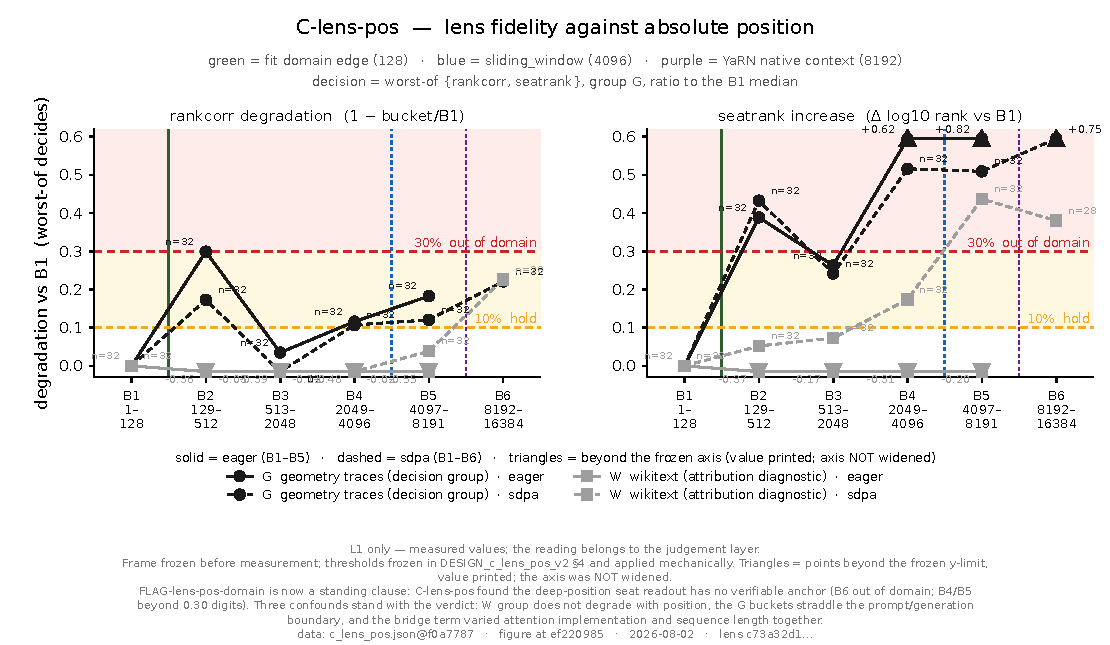
\includegraphics[width=\linewidth]{fig_C1_fidelity_vs_position.pdf}
\caption{\textbf{Lens fidelity against absolute position.} Degradation of
two fidelity measures relative to the first bucket (B1, tokens 1--128),
for the reasoning-trace corpus (G, decision group) and the prose corpus
(W, attribution diagnostic). Left: head-of-distribution rank correlation,
as a ratio to the B1 median. Right: word-group rank deviation, as an
absolute difference in $\log_{10}$ rank. The decision is the worst of the
two, on group G only. Dashed horizontal lines are the pre-registered
thresholds; vertical guides mark the fit-domain edge (128), the sliding
window (4096) and the native context length (8192). The axes, buckets and
decision lines were committed before any measurement existed. Triangles
mark points beyond the frozen limit with the value printed: \emph{the
axis was not widened.}}
\label{fig:c1}
\end{figure}

\begin{figure}[t]
\centering
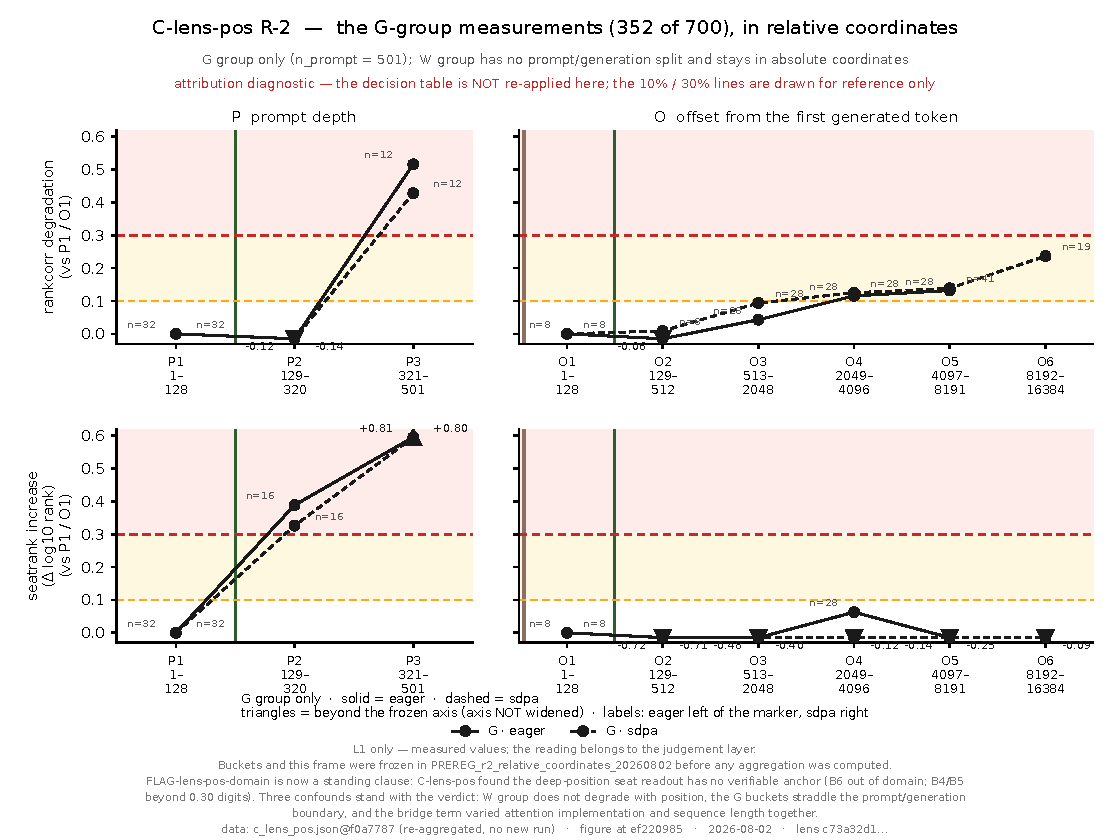
\includegraphics[width=\linewidth]{fig_C2_relative_coordinates.pdf}
\caption{\textbf{The same measurements in relative coordinates.} The
reasoning-trace measurements of Figure~\ref{fig:c1} (352 of the 700),
re-bucketed by depth within the prompt (left column) and by offset from
the first generated token (right column). \textbf{No new model run was
performed.} The prose corpus has no prompt/generation split and stays in
absolute coordinates, so it does not appear here. Baselines are the first
bucket of each coordinate system, not B1. The 10\%/30\% lines are drawn
for reference only; the decision table is not re-applied. Buckets and
this frame were committed before the aggregation was computed.}
\label{fig:c2}
\end{figure}

\subsection{Depth within the prompt, across three prompts}
\label{sec:pdepth}

Within the prompt, the deepest bucket degrades. The initial measurement
saw this on a single prompt read four times, which licensed nothing about
prompts in general. We added two prompts (eight traces over three
prompts) and froze the reading table before the run: with the shallowest
bucket P1 as baseline, ``degraded'' means a rank-correlation drop
$\geq 30\%$ \emph{or} a word-group rank deviation $\geq +0.30$ dex ---
the thresholds of Figure~\ref{fig:c1}, applied mechanically.

\begin{center}
\small
\begin{tabular}{@{}llccccc@{}}
\toprule
& & \multicolumn{2}{c}{Rank correlation} & \multicolumn{3}{c}{Word-group rank deviation} \\
\cmidrule(lr){3-4}\cmidrule(lr){5-7}
Prompt & Length & P2 & \textbf{P3} & P2 & \textbf{P3} & P3, refitted \\
\midrule
1 & 458 & $-72.1\%$ & $\mathbf{+0.4\%}$ & $+2.000$ & $\mathbf{+1.152}$ & $+1.206$ \\
2 & 470 & $-72.1\%$ & $\mathbf{+0.4\%}$ & $+2.000$ & $\mathbf{+0.530}$ & $+0.552$ \\
3 & 501 & $-12.0\%$ & $\mathbf{+51.6\%}$ & $+0.389$ & $\mathbf{+0.812}$ & $+1.011$ \\
\bottomrule
\end{tabular}
\end{center}

\noindent\emph{Prompts 1 and 2 share their first 354 tokens; their P1
baselines and P2 entries are therefore identical by construction, not
independent replicates} (see Limitation~3). The repeated ``$-72.1\%$ /
$+2.000$'' across the two rows is the visible symptom of this. The
pre-registered comparison --- P3 against P1 --- is unaffected: P3 spans
the divergence point at token 354, so all three rows differ there.
The last column (added in v3.2) is the pre-registered P3-against-P1
reading on the refitted lens (Section~\ref{sec:provenance-note}), on the
same frozen grid and threshold; all three rows stay in the degraded
branch, and Controls A and B read identical on both lenses. The bold
columns are the June-lens values and are unchanged.

The pre-registered comparison is P3 versus P1 (bold). The P2 column is
reported as an observation \emph{outside} the pre-registered comparison:
these are measurements on the same frozen grid, and withholding a
non-monotone shape would be selective reporting.

All three prompts fall in the degraded branch. The deep-prompt
degradation is therefore not specific to a single prompt.

\paragraph{Which measure carried the decision.}
For prompts 1 and 2, rank correlation is flat at $+0.4\%$ --- it does not
approach the $30\%$ threshold --- while word-group rank deviation crosses
the $0.30$ dex threshold by factors of 1.8 to 3.8. For prompt 3 both
measures fire. The scope of ``alone'' is therefore two of the three
prompts, across both attention implementations (prompt 3 fires on both
measures: $+51.6\%$ eager, $+42.8\%$ sdpa).

Had we decided on rank correlation alone, two of the three prompts would
have read as undegraded.

The measure that carried the decision is the one added at design time
against a named failure mode: \emph{a lens whose head is faithful and
whose flank is distorted could pass a decision table}
(\S\ref{sec:method}). That failure mode appeared in measurement. We
report this as an occurrence of a hazard we had named, not as a
prediction confirmed --- it was a design rationale, not a registered
prediction with a stake attached.

\paragraph{Shape.}
In two of the three prompts the largest deviation lies in the
\emph{middle} of the prompt (P2) and shrinks toward the end. We therefore
do not use any localization slogan about degradation living at the
prompt's tail; that shape belongs to one prompt. No mechanism is claimed.

\subsection{Instrument checks inside the fit domain}

\label{sec:arms}

\paragraph{Arm A: a positive control.} Five prompts of at most 14 tokens, read on the distributed lens at the head of the sequence --- below the upper edge of the fit domain but, as a later audit of the fitting script showed, entirely inside the band it excludes (60 of 60 read-out positions lie below position 16). Four of the five rows rise under the frozen ordinal predicate (the row whose intermediate is Mars does not, although its rank reaches 4); the sign-flipped control stays above rank $10^4$ (minimum 59{,}337) and the two applications agree.\footnote{Re-acquired in v3.0 (TSD-20260826): the repaired instrument newly observed the same integers (rise 4/5, sign-flip, determinism); the legacy sign-flip minimum 59{,}337 matched bitwise and is kept as an inspection record. See Revision History.} The lens can see a large signal at the head of the sequence; as a positive control, its validity rests on the null and determinism controls that passed in the same run, not on the fit. This was a design premise of version 1.1 and is now a measured control, with that qualification.

\paragraph{Arm B: the filler is not inert.} Each prompt was prefixed with a fixed preface, \emph{Here is a \{ADJ\} question for you to answer:}, for five adjectives, giving 25 forward passes of identical total length. Against the reference adjective, 14 of the 20 variants \emph{fail} the behavioral-invariance gate (11 by a change of the top-1 token, 3 by an answer-probability shift above 0.02). A one-word change in a preface that says nothing about the question is not behaviorally neutral, and so could not have been assumed neutral for the lens either: the gate is not a formality. On the six variants that pass, the per-position spread of the read-out between variants ($\varepsilon_{\mathrm{fill}}$) has a pooled median of 0.057--0.074 dex across the four word groups, a third quartile near 0.14 and a maximum of 0.76--0.79 dex; the tail is why every downstream predicate uses a three-position window rather than a single position. The read-out region of this arm straddles position 16; the gate itself is read at the final position, outside the excluded band.

\paragraph{Arm C: same content, two depths.} The four rising rows were read with the landmark at position 33 and at position 88 (total length at most 102 tokens; both landmarks lie within the fit domain, the no-corridor condition below its lower edge), after a calibration pass that set the degradation-control threshold from the null series ($\tau_{98} = 1{,}666$; the control read 3{,}648 and passed). The landmark-relative onset is identical at the two depths in all four rows --- 3, 2, 3 and 3 positions after the landmark for the rows whose intermediates are spider, Canada, France and Shakespeare --- while the absolute onset moves by exactly the 55 tokens of the translation. We name this landmark-relative onset invariance SameSeat (the read-out keeps its seat relative to the landmark when the prompt is moved), and its qualifiers travel with it: it concerns the onset of read-out only; it was established within the fit domain; on four rows, one filler family and, after the extension below, four in-domain ladder points; and it is an ordinal reading.\footnote{Converted in v3.0 (TSD-20260826) from a supporting clause to a limitation. Version 2 bounded the resolution by ``the lens's order agreement with the model (0.643--0.902, median 0.801)''; that value was measured on fragment-contaminated sets and is not counted.} On the repaired sets (single-token canonical variants; alias best-of over the two two-word sets; point labels excluded by design; word-like pool $N = 70{,}812$; band 26--56), the lens's order agreement with the model over the same 18 reasoning traces, measured separately under a frozen protocol at depths far beyond this campaign's, is 0.456--0.692 (median 0.544); 0.5 is the value a sign-independent reference would give, and the per-trace effective $n$ after tie exclusion ranges from 13 to 7{,}603. The $n = 13$ trace is F5a-2 seed 2 (B-flail; 14 thinking tokens; $\eta = 0.692$, the upper end of the range) and is read together with that $n$; without it the range is 0.456--0.668 (median 0.543; 17 traces). The lower end, 0.456, is F5b-1 seed 2 (B-bind; $n = 7{,}603$) --- a different trace despite the shared seed number. The onset invariance itself rests on its own controls (the Arm C calibration and the population-null bound of the Revision History), not on this agreement. The no-corridor condition differs from the corridor conditions in its first token and lies entirely below position 16, so its comparison is recorded as descriptive and is not part of the statement. Two rows also show a rising window \emph{inside} the corridor, before the landmark (at absolute positions 2 and 18); we register these early windows (CorridorWindow) as an anomaly flag with zero weight and do not read them.

\subsection{Crossing the fit boundary with content held fixed}

\label{sec:results2}

MapFirst ran in two ladders. The first, six rungs from 88 to 242 tokens of corridor (30 measurement passes and 26 new null-control passes, 279 seconds of compute), crosses the upper edge of the fit domain between the rungs at 121 and 132. The second, four rungs from 286 to 484 (20 passes plus 20 controls, 384 seconds), continues to a total length of 498. Every null-control cell in both ladders stayed above rank $10^3$, with a minimum margin of 0.21 dex, and the determinism checks passed. What follows is descriptive wherever the landmark lies beyond 128; we say so once here and again at the table, because the table has the shape of a claim it does not make.

\paragraph{The onset did not move.} In all ten rungs the same four rows rise and the fifth (Mars) does not, as in Arms A and C. In every cell that passes the behavioral-invariance gate against the rung at 88, the landmark-relative onset is unchanged --- 3, 2, 3 and 3 positions for spider, Canada, France and Shakespeare --- from a total length of about 100 tokens to 498 (Table~\ref{tab:mapfirst})\footnote{Re-read in v3.0 (TSD-20260826) in two stages: under the frozen coherence constant 4 --- fitted to the compressed floor of the fragment sets --- the re-run stops at calibration and the row is unreadable there; under a population-null bound derived for the repaired sets ($B_A = 10{,}482$; non-discriminating as a fence, which is registered) the onset 3, 2, 3, 3 is newly observed at both depths and all ten ladder rungs, integer-identical in both lanes. See Revision History.}; the absolute onset follows the landmark by exactly the corridor length. Counting only the four rows that rise, 16 of 20 cells pass the gate in the first ladder and 5 of 16 in the second\footnote{v3.0: the same counts, 16/20 and 5/16, are obtained under the accepted-variant mass (wmass); agreement with the version-2 counts is recorded descriptively only.} (with the non-rising row included, 21 of 25 and 9 of 20); the comparison in the second ladder therefore rests on 5 cells. The cells that fail the gate show the same onset; they are listed in the table but not counted. Inside the fit domain (rungs 110 and 121) this extends SameSeat to four in-domain ladder points; beyond it, the unchanged onset is recorded under branch B4 --- side by side, descriptive, not a calibration.

\paragraph{The behavior drifted.} The gate failures are not noise at the edge of a threshold. All of them in both ladders (4 and 11) are shifts of the answer probability with the top-1 token unchanged; none is a change of top-1. For Shakespeare the shift grows monotonically with depth in the second ladder, $-0.1031$ at 286, $-0.1178$ at 352, $-0.1523$ at 418 and $-0.1676$ at 484, after $+0.0335$ at 110 and $-0.0621$ at 242 in the first; for France it reaches $-0.0616$ at 484; Mars, which never rises, passes at every rung ($|\Delta p| \leq 0.0097$). Under one and the same operation the read-out's onset stayed put while the model's answer probability moved. We record the two side by side and do not identify a mechanism; the predicates and scales of the two observations differ, and neither is evidence about the other.

\paragraph{The instrument's floor thickened.} Two read-outs of the same content at different total lengths need not agree bitwise, because the tensor shapes differ; we measured that floor (ShapeJitter, a shape-dependent difference, not a stochastic one) rather than assuming it. Inside the fit domain (33 against 88) its maximum is 0.045 dex. Across the first ladder the floor stayed thin: 88 against 110 agreed bitwise ($n = 360$), and 88 against 121 and against 132 had median 0 and maximum 0.0974 dex. In the second ladder 286 against 352 again agreed bitwise ($n = 1{,}350$), but every pair involving the rung at 484 read a median near 0.0066 and a maximum of 0.3135 dex\footnote{Re-registered in v3.0 (TSD-20260826): the floor keeps its shape --- in-ladder pairs agree bitwise at the same pairs and the same $n$ (360; 1{,}350); the pairs involving the deepest rung read max 0.3372 dex (L1 max 0.1007); the legacy lane reproduces the version-2 floor exactly. Any comparison at that depth carries the floor.} --- about seven times the in-domain value, and above the 0.30-dex line of version 1.1. The floor itself is a result: any comparison at that depth must carry it, and the in-domain value must not be extrapolated to it.

\paragraph{What the boundary did and did not mark.} The fit boundary at 128 left no seam in the onset, in the null floor (the per-row null minimum is integer-identical from 88 through 154 and changes only at 242, and again only at 484), or in the shape floor up to 242. It did leave a mark in two descriptive statistics that we register without reading: a knee in the phase profile at the deepest rungs (Shakespeare at 242 and at 484; spider at 484, exactly at threshold), and the drift above. Contrasts between adjacent deep bands far from the boundary are small (median 0.007--0.020 dex), so the boundary contrast, where it appears, is not a contrast that appears everywhere. None of this is a guarantee; it is the map on which a next campaign would be planned.

\paragraph{Scope-qualified absence.} We state the outcome in the form we use internally, because the form is the content. Observable: the landmark-relative onset of a three-position window. Depth: up to 484 tokens of corridor (total length 498). Family: one 11-token corridor unit, one model, one lens. Cells: those passing the behavioral-invariance gate, counted above. Within this scope no position-axis degradation was detected. This does not substitute for calibration, and it says nothing about the fidelity of the read-out to the model at that depth.

\begin{table}[t]\centering\small\caption{\textbf{MapFirst: landmark-relative onset across the fit boundary.} Corridor = tokens of filler before the landmark; the rung at 88 is the gate reference. Onset is given for the four rising rows (spider, Canada, France, Shakespeare); the fifth row (Mars) rises at no rung. Gate failures are shifts of the answer probability beyond $0.02$ with the top-1 token unchanged; failing cells show the same onset but are not counted. Rows at or beyond 132 are descriptive by the frozen reading rule (branch B4): an unchanged onset there does not substitute for calibration. (v3.0: rows re-acquired under repaired sets; see Revision History.)}\label{tab:mapfirst}

\begin{tabular}{@{}rp{2.3cm}p{2.1cm}p{7.6cm}@{}}\toprule Corridor & Landmark vs.\ fit domain & Onset (rel.) & Gate failures vs.\ 88 \\ \midrule 88 & inside & 3 / 2 / 3 / 3 & reference \\ 110 & inside & 3 / 2 / 3 / 3 & Shakespeare ($+0.0335$) \\ 121 & inside (window) & 3 / 2 / 3 / 3 & none \\ 132 & beyond & 3 / 2 / 3 / 3 & none \\ 154 & beyond & 3 / 2 / 3 / 3 & France ($+0.0220$) \\ 242 & beyond & 3 / 2 / 3 / 3 & France ($+0.0302$), Shakespeare ($-0.0621$) \\ 286 & beyond & 3 / 2 / 3 / 3 & Shakespeare ($-0.1031$) \\ 352 & beyond & 3 / 2 / 3 / 3 & spider, Canada ($+0.0255$), Shakespeare ($-0.1178$) \\ 418 & beyond & 3 / 2 / 3 / 3 & spider, France ($-0.0248$), Shakespeare ($-0.1523$) \\ 484 & beyond & 3 / 2 / 3 / 3 & spider, Canada ($-0.0350$), France ($-0.0616$), Shakespeare ($-0.1676$) \\ \bottomrule\end{tabular}\end{table}

% =====================================================================
\section{The contribution: a calibration with no anchor}
\label{sec:contribution}

\subsection{No external anchor}

An instrument that reads dispositions has no external oracle.

The lens is designed to read the \emph{potential to verbalize a token in
the future}. The only quantity available to check it against is the
model's final-layer logits --- the prediction of the \emph{next} token.
These two are different by construction. Agreement can therefore be
measured; disagreement cannot be converted into a verdict of failure. A
divergence may be (i) unfaithful extrapolation by the lens or (ii) a
widening --- correct, and expected --- gap between disposition and next
token. This study cannot separate them, and the obstruction is not one of
sample size or compute (Limitation~5).

\subsection{No internal origin}

Nor is there an origin inside.

First, as \S\ref{sec:coords} shows, the choice of baseline cell reverses
the sign of ``degradation'' ($+0.82$ against $-0.14$ dex). Second, as
\S\ref{sec:pdepth} shows, agreement at the head of the distribution does
not imply fidelity at the depth the instrument actually reads: cells
exist in which head correlation is flat while deep ranks alone move the
verdict. Where to place the origin, and at what depth to look, are not
settled from inside the calibration.

This is stronger than an origin one has merely failed to measure. When a
reference has simply been left unmeasured, a matched control recovers it:
one runs the same system without the intervention and reads the
difference. On the position axis there is no such run. There is no
unintervened position, and the prompt head and the generation head are
equally legitimate zeros; no experiment inside this frame chooses between
them. The claim is therefore not that the quantity depends on a
reference --- that much is a familiar property --- but that on this axis
the experiment that would fix the reference cannot be constructed.

\subsection{The statement}

\begin{quote}\Large\itshape
The calibration was anchored neither outside nor inside the instrument.
\end{quote}

\noindent
--- no external oracle to check it against, and no internal origin to
measure from.

This structure is not specific to this lens. Anyone who inherits a
disposition-reading instrument together with its default settings
inherits the same problem. The contribution of this paper is not a
number; it is a name for that problem.

The second campaign does not supply the missing origin, and we want to be exact about why, since its table invites the opposite reading. An onset that stays put when the prompt is moved is a statement about one observable under one operation. It narrows where a position-axis gap could live --- not in this observable, at these depths, in this family --- and it does so without any external oracle, which is its virtue. But invariance is not fidelity: the same campaign watched the model's own answer probability drift and the instrument's floor thicken under the same operation, and it has no way to say which of the three quantities is telling the truth about depth. The map comes first; the instrument's correctness at depth is still not on it.

We do not claim the lens is unusable. On prose it is faithful
(\S\ref{sec:pillars}). The claim is narrower and, we think, more useful:
\emph{readings taken deep inside a reasoning trace have no verifiable
anchor.}

\begin{quote}\large\itshape
Give us a ruler for the order of reasoning.
\end{quote}

% =====================================================================
\section{Limitations}
\label{sec:limits}

\begin{enumerate}\itemsep3pt
\item Single model (OLMo-3-1125-32B), single stack (PyTorch, Apple MPS,
  bfloat16).
\item Single lens (md5 \texttt{c73a32d1\ldots}), single band (layers
  26--56).
\item \textbf{The reasoning-trace corpus is 3 prompts over 8 traces, but
  these are not independent samples, for two reasons.} (a) In a causal
  language model the state at a prompt position depends only on tokens up
  to that position, so multiple traces of one prompt reproduce identical
  values on the prompt side. (b) The three prompts are edit variants
  sharing prefixes (divergence at tokens 86 and 354), so before a
  divergence point, different prompts return \emph{exactly} the same
  value --- we verified this: two pairs of prompts, 13 positions each,
  gave $|\Delta| = 0.0000$ in word-group rank deviation. Consequently the
  correct unit for counting independent values is
  $(\text{prefix},\,\text{position})$, not $(\text{prompt},\,
  \text{position})$ and not the number of rows. Across the three
  prompt-internal buckets the counts are, respectively, rows
  $64/32/24$; $(\text{prompt},\text{position})$ $24/12/9$;
  $(\text{prefix},\text{position})$ $\mathbf{11/8/8}$. We therefore do
  \emph{not} claim to have doubled $n$. The claim is only that positional
  generalization widened from one prefix to three. \emph{Disclosure:} the
  pre-registration froze the distinct count under
  $(\text{prompt},\text{position})$, giving an expected 9; the sharper
  predicate $(\text{prefix},\text{position})$, giving 8, was identified
  after the run. Prefix sharing is a property of causal language models,
  not a defect of the sample.
\item The prose corpus is the lens's own fit dataset, which favors it.
\item \textbf{Fidelity is checked against the model's final-layer logits,
  i.e.\ the next-token prediction, while the lens is designed to read
  near-future disposition.} The two differ by construction. A divergence
  cannot be attributed to (i) unfaithful extrapolation rather than (ii) a
  growing gap between disposition and next token. This is not a shortfall
  of samples or compute: \emph{an instrument that reads disposition has
  no external anchor for correctness.}
\item Position buckets were frozen in absolute coordinates, and in
  reasoning traces they straddle the prompt/generation boundary; the
  re-aggregation in relative coordinates was frozen and committed before
  it was computed.
\item Readings depend slightly on run configuration: ``same prompt, same
  value'' does not hold in general --- agreement requires the run
  configuration to match as well. The magnitude is given in
  \S\ref{sec:method} and is far below the decision threshold; the
  decision is unaffected. Practitioners must fix not only the
  configuration of the model but the configuration of the reading.
\item Traces for the multi-prompt extension were selected by a length
  rule ($>512$ tokens); the distribution over generation-side offsets is
  therefore not an unbiased sample, and we do not read it.
\item The second campaign reads five prompts, one filler family (an 11-token unit repeated) and one kind of operation (translation by prefixing); its in-domain support is four ladder points. Nothing in it is a sample of prompts, fillers or operations, and the onset it reports is the position at which a token becomes readable by this lens, not the time at which anything is computed.
\item Beyond the fit domain the unchanged onset is recorded under a frozen rule (branch B4) as descriptive only. An instrument that did not break out of its domain has not been calibrated there; the scope-qualified absence of Section~\ref{sec:results2} is the strongest form we permit ourselves.
\item The fit domain has a lower edge as well as an upper one: the fitting script excludes positions below 16. Every read-out of Arm A, and part of the read-out region of Arm B, lies inside that excluded band; the first bucket of version 1.1 (tokens 1--128) also contains it. The companion fidelity note bounds the effect of binding to the fit positions at 0.10 dex on prose; we have not measured it on reasoning traces.
\item The behavioral-invariance gate removes cells as depth grows (from 4 of 25 in the first ladder to 11 of 20 in the second). We did not relax the gate to keep cells: the map of which cells remain is itself a result, and a relaxed gate would have hidden the drift it in fact detected.
\item \emph{Revision v3.0 (TSD-20260826):} all rank statements are pool-internal ($N = 70{,}812$) under band 26--56; set-level mass comparisons across sets are not made (the band median of a set mass is nonlinear over subset sums). The word groups of version 2 inherited a first-token rule and are superseded; the values re-acquired under the repaired acceptance are listed in the Revision History section.
\item \emph{Fit environment of the instrument (v3.2).} A lens artifact encodes the forward it was fitted on. The June artifact encoded a forward that the library had already corrected by the time we read it, and nothing in the artifact said so; the hash we pinned identified the file, not the forward. Our provenance discipline now records the fit environment of every instrument (\texttt{provenance} in the refitted artifacts; the transformers version and commit of the fitting run), and we recommend the same to any reader inheriting a distributed lens (Section~\ref{sec:provenance-note}).
\item On the refitted lens the \texttt{sdpa} cells of the reasoning-trace corpus rest on $n = 16$ positions from two texts (June lens: $n = 32$ from four), because two of the four long traces (about 16k tokens) could not be measured under \texttt{sdpa} on the current platform (macOS 27.0, Metal: the process terminates), so \texttt{sdpa} values of the refitted lens --- such as the B4 rank-correlation degradation of $+0.382$ --- are two-text values and are reported beside the \texttt{eager} values, which remain primary.
\end{enumerate}

% =====================================================================
\section{Research workflow and AI involvement}
\label{sec:workflow}

This calibration was carried out through a two-layer workflow of large
language models~\cite{anthropic2026claude}, described here because parts
of it are load-bearing for the paper's warrant. An \emph{execution layer}
(agentic coding interface) implemented the harness, ran the measurements,
and reported them in frozen documents. A separate \emph{judgment layer}
(chat interface) performed adversarial review of every design and result
document under a single-identified-fatal-flaw discipline, and froze the
pre-registrations and reading tables. The two layers are separated by a
deliberate information asymmetry: the judgment layer has no access to the
codebase, the raw outputs, or the subject model, and reads only the
frozen documents.

Three boundaries fix responsibility. First, the subject of measurement is
OLMo-3-32B and the released lens; no workflow model is a measurement
subject. Second, no language model adjudicates an outcome: every
quantitative verdict is taken against a threshold frozen before its
measurement and applied mechanically. Third, every load-bearing decision
--- thresholds, terminology, framing, and the final wording of the claim
--- was reserved to and made by the human author, who reviewed all frozen
documents and bears sole responsibility for every claim.

The workflow's own errors are reported rather than removed. Two are
material to this paper. The scope of the prose finding
(\S\ref{sec:pillars}) was dropped by the execution layer in a draft and
restored in review after collision with the ledger. The sharper counting
predicate in Limitation~3 was identified only after the run, and is
disclosed as such rather than presented as pre-registered.

The second campaign followed the same protocol, with the same separation between execution and judgment, and its errors are likewise reported rather than removed. One run was halted by its own calibration control before measurement and re-run after the control threshold was re-derived from the null series; the halt and the re-derivation are both on record. One registered prediction failed: the pre-registration of the first ladder predicted that behavior would pass the gate at every rung, and it did not in four cells; the miss is charged to the judgment layer and kept. One headline count in the second ladder was written by hand as 12 of 20 and corrected to 11 of 20 when the judgment layer's review forced a recount from the output file; the correction is recorded in place with the sweep that found it, and the number in this paper is the recounted one.


% =====================================================================
\section*{Revision History (v3.0 / v3.1 / v3.2, REVISION-ID: TSD-20260826)}
\label{sec:revision}

\noindent\textbf{Registered:} 2026-08-26. \textbf{Values:} 2026-08-26/27/28.
\textbf{Instrument (archived):} joshaku v1.2.0~\cite{joshaku2026} (seven
modules, combined md5 \texttt{89b194be...}; 20 tests; archived at doi:
10.5281/zenodo.22218669), SPEC v1.2 (md5 \texttt{e95f4661...}, included in
that record); calibration tests as in the registry.
\textbf{Instrument (as run; declared in v3.1):} the five arm, ladder and
null outputs (\texttt{arm\_a\_v3}, \texttt{arm\_c\_v3}, \texttt{cii\_l1\_v3},
\texttt{cii\_l2\_v3}, \texttt{cii\_nulls\_v3}) record in their \texttt{meta}
the joshaku state they ran under: combined md5 \texttt{2bb7fe6c...} (source
commit \texttt{ad24326a}, 2026-08-26; 19 tests; SPEC v1.1, md5
\texttt{85715fe0...}), the state one commit before the v1.2.0 freeze
(2026-08-27). The two states differ in one module only, \texttt{ranks.py},
to which v1.2.0 added two alias helpers (\texttt{alias\_best\_of},
\texttt{alias\_pair}) and their exception class; the modules these runners import (\texttt{pgrain},
\texttt{masks}) are byte-identical between the two states and no existing
function changed, so no recorded value depends on the difference. The
shape-floor and order-agreement outputs (\texttt{r211\_v3},
\texttt{f5\_corr\_v3\_*}) do not record a fingerprint --- a provenance gap,
registered as such; both post-date the freeze by commit date, and the
order-agreement runner imports \texttt{alias\_pair}, which exists only from
v1.2.0. Tokenizer pin:
\texttt{allenai/}\allowbreak\texttt{Olmo-3-1125-32B}\allowbreak\texttt{@c2b61dae...}; lens
\texttt{Olmo-3-1125-32B\_jacobian\_lens.pt}; word-like pool $N = 70{,}812$;
layer band 26--56 (one layer narrower than the CommitStage band --- the two
are not interchangeable).
\textbf{What happened:} the reading sets used here contained sub-word
fragments (spider $\to$ `sp', Shakespeare $\to$ `Sh', insect $\to$ `in'),
an instance of the pre-registered first-token rule now registered as a
defect (T1). All sets were rebuilt (single-token canonical variants; drops
registered) and the affected measurements re-acquired. During
re-acquisition the runner's universe assertion caught a wrongly declared
model before any measurement (Qwen declared, OLMo intended); the corrected
run is the one reported.

\subsection*{Part I --- Readings}

\begin{center}\small
\captionof{table}{Revised readings (v3.0). (a)-type = old values excluded from
evidence and the same integers newly observed; (c) = unreadable as frozen.}
\label{tab:revision}
\begin{tabular}{@{}p{3.1cm}p{2.4cm}p{8.6cm}@{}}\toprule
Row & Reading & Note text \\ \midrule
Arm A (rise 4/5, sign-flip, determinism) & (a)-type & Old values are excluded from evidence; the repaired instrument newly observed the same integers (the legacy sign-flip value 59{,}337 matched bitwise and is kept as an inspection record). \\
SameSeat onset (3, 2, 3, 3) & two-stage & Stage one: under the frozen coherence constant 4 --- a constant fitted to the compressed floor of the fragment sets --- the re-run stops at calibration and the row is unreadable there. Stage two: under a population-null bound derived for the repaired sets ($B_A = 10{,}482$; as a fence it is non-discriminating, which is registered), the onset (3, 2, 3, 3) is newly observed at both depths and all ten ladder rungs, integer-identical in both lanes. \\
Gate passages & new scale & 16/20 and 5/16 under the accepted-variant mass (wmass); agreement with the old counts is recorded in the descriptive column only. \\
MapFirst onset rows & (a)-type, readable rows only & At the second ladder the readable rows are P3 and B1 (P2 has one eligible cell; P5 none --- (c)). \\
Null controls, $\tau_{98}$ & re-derived & Values are not compared across instruments. \\
ShapeJitter floor & new registration & The floor keeps its shape: in-ladder pairs agree bitwise at the same pairs and the same $n$ as before (360; 1{,}350); the pairs involving the deepest rung read max 0.3372 dex (L1 max 0.1007); the legacy lane reproduces the old floor exactly. Any comparison at that depth carries the floor. \\
\bottomrule\end{tabular}
\end{center}

\subsection*{The order-agreement clause (conversion from support to limitation)}

The sentence of version 2 that bounded SameSeat's ordinal resolution by
``order agreement 0.643--0.902 (median 0.801)'' is converted in
Section~\ref{sec:arms} (Arm C) from a supporting clause to a limitation:
on the repaired sets the agreement over the same 18 traces is 0.456--0.692
(median 0.544), against 0.5 for a sign-independent reference; the per-trace
effective $n$ after tie exclusion is 13 to 7{,}603, with the $n = 13$ trace
(F5a-2 seed 2; $\eta = 0.692$, the upper end) named in place and the range
without it (0.456--0.668; median 0.543; 17 traces) given beside it. The
previously printed value was measured on fragment-contaminated sets and is
not counted. \textbf{Dependency table (machine-checked):} the old clause is
cited by exactly one sentence in the paper (the SameSeat resolution
qualifier); no verdict elsewhere stands on it; the registration of SameSeat
under the population-null bound contains no reference to the agreement.
Legacy replication: all 18 per-trace legacy values reproduced the registered
ones at $\Delta = 0.0$.

\subsection*{Instrument section}

\begin{itemize}\itemsep2pt
\item Set repair: fragments `sp' / `Sh' / `in' removed by acceptance, not
by filtering; every dropped variant is registered.
\item Universe correction history: one mis-declared universe was caught by
the $N$ assertion before measurement; the inspection card prints the
universe and the tokenizer sha.
\item Calibration record for the order-agreement values: controls for the
F5a-2 half were re-run after the fact (determinism; per-trace replication
$\Delta = 0.0$; sign-flip identity on single-id sets, exact for both
variants, 4/4 each). The two-id identity control originally specified is
non-informative by construction (best-of over two ids turns a minimum into
a maximum under negation) and is replaced in the calibration record; the
values themselves are unchanged.
\item Coherence door: under a population null, four-word-set floors span
two to four orders of magnitude, so a common $\tau_{98}$ across sets is a
design question for a separate program (flag).
\item Environment: integer rank series reproduce across environments
(bitwise ladder pairs; 18/18 order-agreement legacy values at
$\Delta = 0.0$); the lens's $10^{-6}$-scale masses do not. Mass-lane
citations carry this line.
\end{itemize}

\noindent\textbf{Limitations (one line):} all rank statements are
pool-internal ($N = 70{,}812$) under band 26--56; set-level mass comparisons
across sets are not made (nonlinearity of band medians over subset sums).
\textbf{Revision history:} v2 (2026-08-21, doi: 10.5281/zenodo.22041724) ---
superseded readings marked inline; v3.0 (2026-09-01, doi:
10.5281/zenodo.22219346) --- TSD-20260826; v3.1 (2026-09-11, doi:
10.5281/zenodo.22701008) --- declares the as-run instrument fingerprint; no
value changed; v3.2 (this version) --- see below.
% v3.2 DOI: 10.5281/zenodo.22928237 (reserved on the paper record 2026-09-24; live on publication)
Inspection records: READCARD md5s R2v2 \texttt{64b7ea9d} / R2b
\texttt{5980f44c} / R4 \texttt{14123f9c}; scope table and equivalence check
(R4-a) in the registry. The re-acquisition runners and their outputs
(Arms A/C, both ladders, the shape floor and the order-agreement lanes) are
released with the package (\REPOURL{}; concept DOI 10.5281/zenodo.21768364,
version 3.1.0 or later).

\noindent\textbf{v3.2 (2026-09-23).} Adds the instrument-provenance note
(Section~\ref{sec:provenance-note}; the June lens was fitted under
transformers 5.11.0 with YaRN applied to sliding-window layers; read-outs
ran on 5.14.1) and places the readings of the refitted lens (2026-09-21,
sha256 \texttt{c6ee7d22\ldots}) beside the June readings in the coordinate
table, the multi-prompt table (Section~\ref{sec:pdepth}) and the released data. No value is withdrawn; no
verdict of the frozen decision table changes.

% =====================================================================
\section*{Data and code availability}

All measurements are released with per-position values retained: the main
run (700 measurements), the control re-measurement, the relative-coordinate
re-aggregation (no new run), and the multi-prompt extension (224
measurements), together with the determinism and neutrality checks. The
measurement code imports the lens, the word groups, the rank computation
and the token mask verbatim from the upstream implementation.\footnote{The inherited word groups represented a multi-token word by its first token (spider $\to$ `sp', Shakespeare $\to$ `Sh', insect $\to$ `in'); registered as defect T1 in v3.0 and replaced by the acceptance instrument joshaku~\cite{joshaku2026} (Revision History).} The frozen
documents --- the decision table and the two pre-registrations --- are
released with their commit timestamps, which are the evidence that the
freeze preceded the measurement --- as post-hoc English renderings, with the
Japanese originals fixed by \texttt{sha256} (see \texttt{PROVENANCE.md} in the
release). Figure scripts are included and produce an empty frame when no data
file is present.
The second campaign's artifacts --- the per-cell read-outs of Arms A, B and C and of both MapFirst ladders, the null ledgers, the gate tables and the pre-registrations with their commit timestamps --- are released with this version in the same package, under the same manifest discipline.

The package is available at \REPOURL{}\DOICLAUSE{}. Every file is listed in
\texttt{MANIFEST.json} with its \texttt{sha256} both as it ran and as
released, together with an enumeration of every substitution made for
release.

% =====================================================================
\section*{Acknowledgment}

This work was supported by JSPS KAKENHI Grant Number JP26K06399.
A participant in the public discussion of the released artifacts
independently identified the fitting-script default path (Aug.~2026),
which the revised text incorporates.
Manuscript text was drafted within the two-layer workflow described in
\S\ref{sec:workflow}~\cite{anthropic2026claude}; all claims, thresholds
and final wording are the author's.

% =====================================================================
\begin{thebibliography}{9}

\bibitem{gurnee2026workspace}
W.~Gurnee, N.~Sofroniew, A.~Pearce, M.~Piotrowski, I.~Kauvar, R.~Chen,
A.~Soligo, P.~Bogdan, E.~Ong, R.~Wang, T.~B.~Thompson, D.~Abrahams,
S.~Kantamneni, E.~Ameisen, J.~Batson, and J.~Lindsey,
``Verbalizable representations form a global workspace in language
models,'' \emph{Transformer Circuits Thread}, Jul.~6, 2026. [Online].
Available: \url{https://transformer-circuits.pub/2026/workspace/}

\bibitem{merity2017wikitext}
S.~Merity, C.~Xiong, J.~Bradbury, and R.~Socher, ``Pointer sentinel mixture
models,'' in \emph{Proc. ICLR}, 2017.

\bibitem{nostalgebraist2020logitlens}
nostalgebraist, ``Interpreting GPT: the logit lens,'' LessWrong, 2020.
[Online]. Available:
\url{https://www.lesswrong.com/posts/AcKRB8wDpdaN6v6ru/interpreting-gpt-the-logit-lens}

\bibitem{olmo3}
Allen Institute for AI, ``OLMo-3-1125-32B,'' 2025. [Online]. Available:
\url{https://huggingface.co/allenai/Olmo-3-1125-32B}

\bibitem{fidelityeight2026} M.~Higashida, ``FidelityEight: Frozen-protocol fidelity measurements of the distributed Jacobian-lens checkpoints,'' Zenodo, Aug.~2026. doi: 10.5281/zenodo.21990390.

\bibitem{joshaku2026} M.~Higashida, ``joshaku: token-set acceptance for lens readouts, fixed before any run (v1.2.0),'' Zenodo, Sep.~2026. doi: 10.5281/zenodo.22218669.

\bibitem{anthropic2026claude}
Anthropic, ``Claude (large language model family),'' 2026. [Online].
Available: \url{https://claude.ai}. Used as research-workflow execution
and judgment layers and for manuscript drafting; see
\S\ref{sec:workflow} and Acknowledgment.

\end{thebibliography}

\end{document}
